\documentclass{scrartcl}

% importations de packages utiles
\usepackage[backend=biber, style=alphabetic]{biblatex}
\addbibresource{rng.bib}
\usepackage[utf8]{inputenc}  % pouvoir écrire avec des accents
\usepackage[french]{babel}  % francophopnie
\usepackage{amsmath, amssymb}
\usepackage{hyperref}  % liens clicables dans pdf final
\usepackage{tikz}  % pouvoir tracer des dessins sympas
\usepackage{listingsutf8}  % rendu de "code" (avec config ci-dessous)
\definecolor{lstcolor}{rgb}{0.9,0.95,0.95}
\definecolor{lstcommentcolor}{rgb}{0.,0.2,0.}
\lstset{
  frameround=tttt,
  %autogobble,
  frame=single,
  backgroundcolor=\color{lstcolor},
  % extendedchars=true,
  % basicstyle=\ttfamily\small,
  keywordstyle=\bfseries\color{blue},
  identifierstyle=\bfseries\color{red},
  stringstyle=\bfseries\color{orange},
  commentstyle=\color{lstcommentcolor},
  language=Python,
  keepspaces=True,
  basicstyle=\fontfamily{pcr}\selectfont\small, % monospace it for copypasting
  upquote=true,
  columns=flexible,
  showstringspaces=False,
  literate={é}{{\'e}}1
}
\begin{document}

\section{Les générateurs à congruence linéaire}
\subsection{Introduction}
Le générateur à congruence linéaire est un générateur de nombres aléatoires qui a été mis au point en 1949 par Derrick Lehmer. Elle est basée sur une fonction linéaire et l'arithmétique modulaire. Cela en fait une méthode déterministe dont la période dépend dans une large part de ses paramètres.
Le caractère déterministe a pour intérêt la reproductibilité des résultats permettant d'une part la recherche d'erreur dans les codes et d'autre part comme référence pour des résultats scientifiques.
Une suite $(X_n)$ de nombres est produite par itération à partir d'une graine:
$X_{n+1} = (a X_n +c)[m]$
Où $[m]$ est le module m \\
a le multiplicateur \\
c l'incrément \\
et $X_0$ la graine. \\

La division entière dans la formule permet d'obtenir le reste de la division entière. Ainsi, à partir de la graine, chaque nombre peut être un entier entre 0 et $m-1$.
Par conséquent, dans le meilleur des cas, $m$ nombres sont produits et la suite se répète.
Un enjeu est donc de choisir un module suffisamment grand de sorte d'avoir une suite de nombres longue.

\subsection{Choix des paramètres}
La conjugaison des paramètres $a$, $c$ et $m$ est donc décisive dans le caractère aléatoire de la suite générée. Ceci est illustré sur des exemples simples:

1er cas:\\
$X_{n+1} = (3 X_n +2)[5]$ avec $X_0 = 1$ donne pour suite $[1,0,2,3,1,..]$ et la période est de 4.
2ème cas:\\
$X_{n+1} = (4 X_n +2)[9]$ avec $X_0 = 4$  donnant $[4,0,2,1,6,8,7,3,5,4]$ avec une période de 9 qui est maximale.
Ainsi, le choix des paramètres obéit à des critères qui rendent maximale la période dénommés usuellement "magic numbers".
D'autre part, on a pu remarque dans le premier cas que le nombre 4 est absent de la liste. S'il avait été donné comme graine, la période aurait été de 1 avec uniquement pour sortie la valeur 4.

En conclusion, la combinaison de paramètres permet une grande variété de résultats mais ne doit pas occulter l'importance de la graine pour obtenir des nombres les plus aléatoires possibles.

\subsection{Des générateurs à congruence linéaire types}
Il existe un spectre important de générateurs utilisés dans tous les langages. Citons en particulier les cas suivants:
Fonction RANDU d'IBM : $X_{n+1} =65539 X_{n} [2^{31}]$\\
Turbo Pascal : $X_{n+1} =(129 X_{n} + 907633385)[2^{32}]$\\
Fonction \textit{ rand()} (C ANSI) : $X_{n+1} =(1103515245 X_{n}+12345) [2^{31}]$\\
où le module est de l'ordre de 32 bits à la limite maximale des ordinateurs utilisés.

\subsection{Tests de validité}
Afin de tester la validité des du générateur on peut effectuer un \textit{ test spectral}. Celui-ci permet d'observer directement la corrélation de la suite de nombres.
Il s'agit de représenter les nombres les uns en fonction des autres dans un espace multidimensionnel de façon à identifier les redondances.
Le générateur $X_{n+1} =(7 X_{n})[101]$ donnent un histogramme des 101 premiers nombres avec la graine $X_0 = 1$ sur la figure ci-dessous à gauche:
\begin{figure}
    \begin{center}
    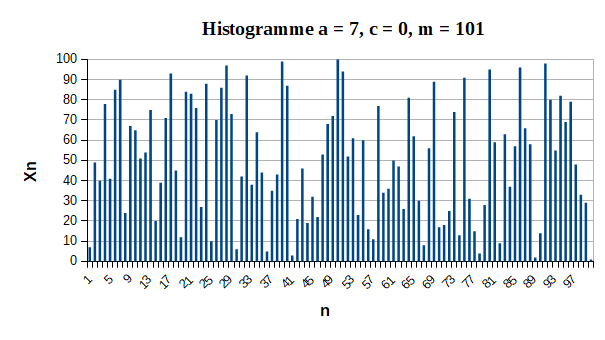
\includegraphics[scale=0.4]{histo7Xn[101].png}
    \hspace{0.1\textwidth}
    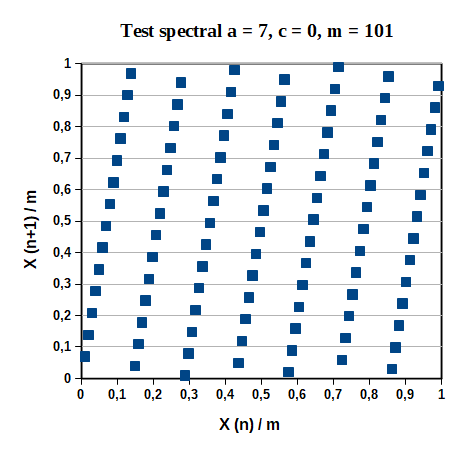
\includegraphics[scale=0.4]{a7m101.png}
    \end{center}
  \end{figure}
Cet histogramme montre la présence de toutes les valeurs possibles sans période inférieure à la valeur du module.
Afin de mettre en évidence les corrélations, on trace les 101 premières paires consécutives de nombres ($X_n/m$,$X_{n+1}/m$). Chaque nombre est normalisé par le module permettant de visualiser dans l'espace $[0,1]^2$.
Sur la figure de droite, on y constate le recouvrement des valeurs entre 0 et 1. Le caractère déterministe apparaît avec les points à distance régulière suivent des droites. De plus, plus cette distance est faible plus le recouvrement est important.

\end{document}